\documentclass[12pt]{article}
\usepackage{graphicx}
\begin{document}
\title{"Quick-and-Dirty" implementation of the exponential function}
\author{C. S. Overgård}
\date{June 2021}
\maketitle
\section{Math}
An 'exponential function' is any fucntion with the general form:
  \begin{equation}
\label{eq:GenEXP}
f(x)=ab^x
	\end{equation}
When refering to \textit{the} exponential funtion it is one which base is the constant \textit{e} (approximatly eqaul to 2.71828). This special exponential function is unique as the derivative of the fucntion is the function itself.
  \begin{equation}
\label{eq:dxEXP}
\frac{d}{dx} e^x = e^x
  \end{equation}
Additionally the exponential function is often used to describe a function whose growth rate depens on its value.
\subsection{Approximations}
When Computing the exponential function a number approximations can be used. The most famouse one being the Taylor expansion of the exponential function
\begin{equation}
\label{eq:TaylorEXP}
e^x \approx 1 + x + \frac{x^2}{2!}+\frac{x^3}{3!}+\frac{x^4}{4!}...
\end{equation}
This function can be simplified to the "Quick-and-Dirty" approximation
\begin{equation}
\label{eq:QnD}
e^x \approx 1 + x(1+\frac{x}{2}(1+\frac{x}{3}(1+\frac{x}{4}(1+\frac{x}{5}...(1+\frac{x}{n})))...)
\end{equation}
Where increases in \textit{n} increases the accuracy of the approximation (for the pourpose of this report 10 is more than adequate). It is obvious that mulitplying everything into the parentheses one returns at Eq.~(\ref{eq:TaylorEXP}). To determine the accuracy of the "Quick-and-Dirty" approximation the result of the function have been plotted against the \textit{exp(x)} function from "\textit{math.h}". The resulting graph can be found in section \textbf{2}. The "Quick-and-Dirty" function also includes a inbuilt statement which reduces the value given to the function. This is done as the Taylor expansion, on which the "Quick-and-Dirty" function is based, is accurate at smaller \textit{x} values.
\pagebreak
\section{Figures}
\begin{figure}[h]
  \centering
  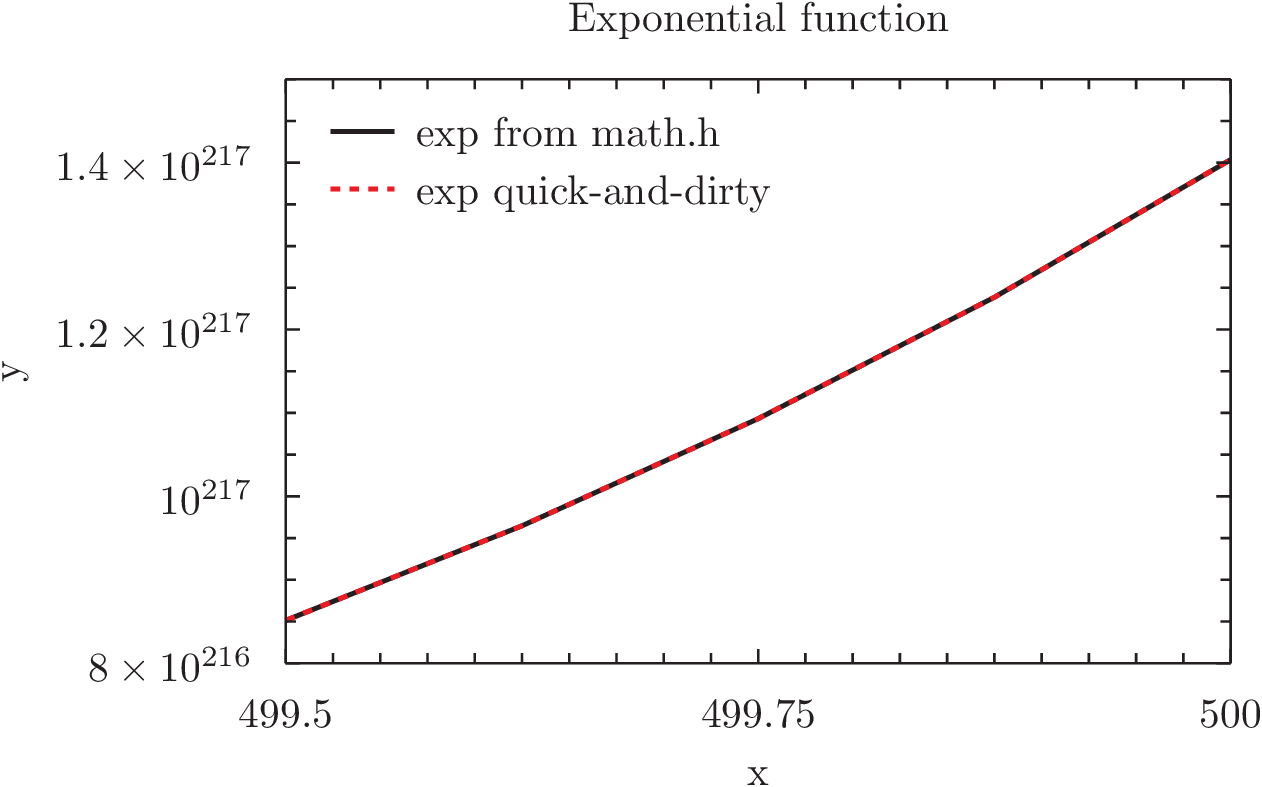
\includegraphics{exp.pyxplot.png}
  \caption{Exponential fucntion (black) compare
  with the "Quick-and-Dirty" implementation (red)~(\ref{eq:QnD})}
  \label{fig:EXP_Pyxplot}
\end{figure}

\end{document}
